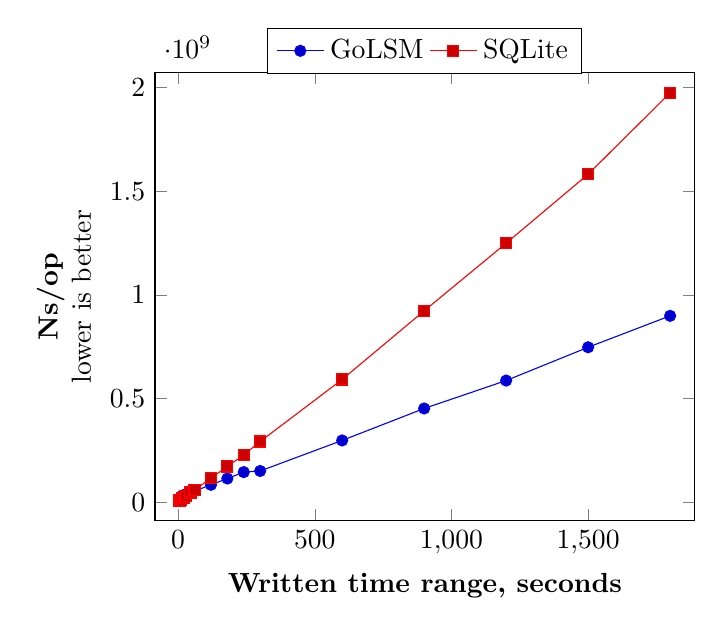
\begin{tikzpicture}
        % first provide your data as table, so later the data can
        % easily be accessed for various stuff
        \pgfplotstableread{
            x    y  z
5 15645901			    9353729
10 22956983			    11181460
15 32283634			    19307910
20 34011973			    21123025
25 33267746			    28927692
30 39930080			    30805858
45 49632256			    47978279
60 54524124			    59648520
120 84668307			    116531430
180 115137807			    173160076
240 146032654			    228964797
300 151417281			    293465746
600 298689957			    592581370
900 452684093			    923305824
1200 587385346			    1249406072
1500 747870163			    1582051745
1800 899311404			    1974174575

        }{\data}
    \begin{axis}[
        x tick style={/pgf/number format/1000 sep=},
	    ylabel style={align=center},	
	    ylabel = \textbf{Ns/op}\\lower is better,
	    xlabel style={align=center},	
	    xlabel = \textbf{Written time range, seconds},
	    enlargelimits=0.05,
	    legend style={
	        at={(0.5,1.1)}, anchor=north,legend columns=-1
	    },
    ]
        % then your `\addplot commands change to
        \addplot table [x=x,y=y] {\data};
        \addlegendentry{GoLSM}
        \addplot table [x=x,y=z] {\data};
        \addlegendentry{SQLite}
    \end{axis}
\end{tikzpicture}